\documentclass{ximera}

\title{Som van vectoren}
%\author{Daan Lipkens} %van wiskunde op maat Sint-Pieterscollege

\begin{document}
\begin{abstract}
    De samenstelling van twee of meer vectoren en de cosinusregel.
\end{abstract}
\maketitle

Twee vectoren van dezelfde grootheid met hetzelfde aangrijpingspunt kunnen opgeteld worden met als resultaat een nieuwe vector. Deze vector wordt \textbf{de resultante} genoemd. 

\section{Grafisch}
Grafisch (kwalitatief) bekomt men de resultante via de kopstaartmethode of parallellogrammethode.  

%---------------------------
% AFBEELDING: Som parallellogram
\begin{figure}[ht!]
    \captionsetup{width=0.85\textwidth}
    \begin{center}
        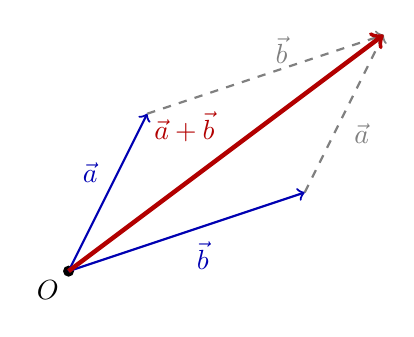
\begin{tikzpicture}[scale=1]
            \coordinate (O) at (0,0); 
            \coordinate (A) at (1,2); 
            \coordinate (B) at (3,1); 
            \coordinate (C) at (4,3); % A + B
            
            \fill (O) circle (2pt) node[below left]{$O$};
            
            \draw[->, thick, blue!70!black] (O) -- (A) node[midway, above left]{$\vec{a}$};
            \draw[->, thick, blue!70!black] (O) -- (B) node[midway, below right]{$\vec{b}$};
            
            \draw[->, dashed, thick, gray] (A) -- (C) node[midway, above right]{$\vec{b}$};
            \draw[->, dashed, thick, gray] (B) -- (C) node[midway, below right]{$\vec{a}$};
            
            \draw[->, ultra thick, red!70!black] (O) -- (C) node[midway, above left]{$\vec{a} + \vec{b}$};
        \end{tikzpicture}
    \end{center}
    \caption{De optelling van twee vectoren via de parallellogrammethode.}
    \label{fig:som_vectoren}
\end{figure}
%---------------------------

\section{Met getallen}
De \textbf{grootte van de resultante} (kwantitatief) kan op verschillende manieren bepaald worden. Erg belangrijk hierbij is om de meetkundige samenstelling in het oog te houden en zeker niet blindelings de groottes van de gegeven vectoren op te tellen! 

In evenwijdige of loodrechte gevallen zijn er efficiënte manieren om de resultante te bepalen (gewone som/verschil of de stelling van Pythagoras). De meest algemene methode is echter de cosinusregel voor de lengte van $\vec{c} = \vec{a} + \vec{b}$:

\[ \| \vec{a} + \vec{b} \|^2 = \| \vec{a} \|^2 + \| \vec{b} \|^2 + 2 \cdot \|\vec{a}\| \cdot \|\vec{b}\| \cdot \cos(\alpha) \]

met $\alpha$ de hoek tussen $\vec{a}$ en $\vec{b}$.

\begin{figure}[ht!]
    \captionsetup{width=0.85\textwidth}
    \begin{center}
        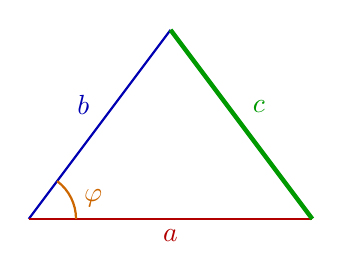
\begin{tikzpicture}[scale=1.2]
            \coordinate (O) at (0,0);
            \coordinate (A) at (3,0);
            \coordinate (B) at (1.5,2);
            
            \draw[thick, blue!70!black] (O) -- (B) node[midway, above left] {$b$};
            \draw[thick, red!70!black] (O) -- (A) node[midway, below] {$a$};
            \draw[ultra thick, green!60!black] (A) -- (B) node[midway, above right] {$c$};
            
            \draw[thick, orange!80!black] (0.5,0) arc (0:53.1:0.5) node[midway, right=1pt] {$\varphi$};
        \end{tikzpicture}
    \end{center}
    \caption{In een gesloten driehoek gebruik je de overstaande hoek $\varphi$ met een \textbf{minteken}.}
\end{figure}

\begin{question}
    Denk na over deze drie bijzondere gevallen:
    \begin{itemize}
        \item Hoe vereenvoudigt de cosinusregel als $\vec{a}$ en $\vec{b}$ \textbf{loodrecht} op elkaar staan? 
        \item Hoe vereenvoudigt de cosinusregel als $\vec{a}$ en $\vec{b}$ \textbf{dezelfde richting en dezelfde zin} hebben? 
        \item Hoe vereenvoudigt de cosinusregel als $\vec{a}$ en $\vec{b}$ \textbf{dezelfde richting en tegengestelde zin} hebben? 
    \end{itemize}
\end{question}

\begin{remark}[foldable=true,title={Twee versies van de cosinusregel?}]\nl
    Er bestaan twee versies van de cosinusregel. Beide formules zijn wiskundig 100\% correct, maar ze gebruiken een \textbf{andere hoek}. Het is cruciaal om te begrijpen in welke situatie je welke formule (en dus welk teken) gebruikt.

    \textbf{1. De klassieke wiskundige cosinusregel (in een driehoek)} \\
    In de wiskunde pas je de cosinusregel toe op de zijden van een gesloten driehoek. Je gebruikt hierbij de \textbf{overstaande, inwendige hoek} $\varphi$ (tegenover de zijde $c$ die je wil berekenen).
    \[ c^2 = a^2 + b^2 \mathbf{-} 2ab\cos(\varphi) \]
    
    \begin{center}
        \captionsetup{width=0.85\textwidth}
        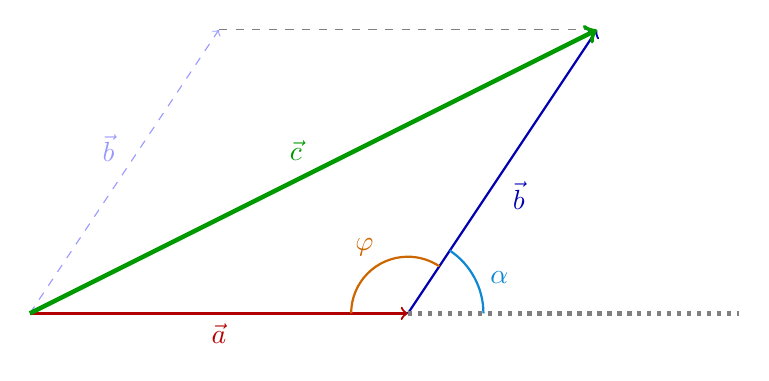
\begin{tikzpicture}[scale=1.2]
            \coordinate (O) at (0,0);
            \coordinate (A) at (4,0);
            \coordinate (B) at (2,3);
            \coordinate (C) at (6,3); % Punt van C = A + B
            
            % Oorspronkelijke b-vector als referentie (staart-aan-staart)
            \draw[->, dashed, blue!40] (O) -- (B) node[midway, above left] {$\vec{b}$};
            \draw[dashed, gray] (B) -- (C);
            
            % Kopstaart optelling (de fysieke driehoek)
            \draw[->, thick, red!70!black] (O) -- (A) node[midway, below] {$\vec{a}$};
            \draw[->, thick, blue!70!black] (A) -- (C) node[midway, below right] {$\vec{b}$};
            \draw[->, ultra thick, green!60!black] (O) -- (C) node[midway, above left] {$\vec{c}$};
            
            % Stippellijn: verlengde van vector a (hulplijn)
            \draw[dotted, ultra thick, gray] (A) -- (7.5,0);
            
            % Hoeken aan knooppunt A
            % De vectorhoek alpha (buiten de driehoek)
            \draw[thick, cyan!70!blue] (4.8,0) arc (0:56.3:0.8) node[midway, right=2pt] {$\alpha$};
            % De inwendige driehoekshoek phi
            \draw[thick, orange!80!black] (3.4,0) arc (180:56.3:0.6) node[midway, above left=-1pt] {$\varphi$};
        \end{tikzpicture}
        \captionof{figure}{Door vector $\vec{b}$ te verschuiven (kopstaartmethode) ontstaat een driehoek. De verlengde hulplijn toont duidelijk dat de inwendige hoek $\varphi$ het supplement is van de vectorhoek $\alpha$. De algemene cosinusregel $c^2 = a^2 + b^2 - 2ab\cos(\varphi)$ gebruikt deze inwendige hoek $\varphi$.}
        \label{fig:cosinus_optelling_hulplijnen}
    \end{center}

    \textbf{2. De vectoriële cosinusregel (in de fysica)} \\
    Wanneer we twee vectoren optellen, plaatsen we deze met hun aangrijpingspunten in de oorsprong (staart-aan-staart). De hoek die we in de fysica standaard kennen, is de hoek $\alpha$ \textbf{tussen de twee vectoren}. 
    \[ \|\vec{c}\|^2 = \|\vec{a}\|^2 + \|\vec{b}\|^2 \mathbf{+} 2\|\vec{a}\|\|\vec{b}\|\cos(\alpha) \]
    
    \begin{center}
        \captionsetup{width=0.85\textwidth}
        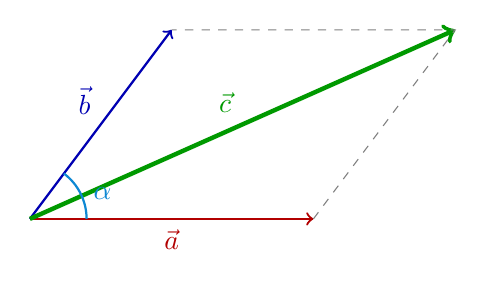
\begin{tikzpicture}[scale=1.2]
            \coordinate (O) at (0,0);
            \coordinate (A) at (3,0);
            \coordinate (B) at (1.5,2);
            \coordinate (C) at (4.5,2);
            
            \draw[->, thick, red!70!black] (O) -- (A) node[midway, below] {$\vec{a}$};
            \draw[->, thick, blue!70!black] (O) -- (B) node[midway, above left] {$\vec{b}$};
            \draw[->, ultra thick, green!60!black] (O) -- (C) node[midway, above left] {$\vec{c}$};
            
            \draw[dashed, gray] (A) -- (C) -- (B);
            
            \draw[thick, cyan!70!blue] (0.6,0) arc (0:53.1:0.6) node[midway, right=1pt] {$\alpha$};
        \end{tikzpicture}
        \captionof{figure}{Bij vectoren gebruik je de ingesloten hoek $\alpha$ met een \textbf{plusteken}.}
    \end{center}

    \begin{hint}\nl
        In de wiskunde gebruik je de cosinusregel met een minteken: $c^2 = a^2 + b^2 \mathbf{-} 2ab\cos(\varphi)$. In de fysica gebruiken we vaak het plusteken. Dit verschil is logisch te verklaren als we kijken naar het \textbf{parallellogram} dat de vectoren vormen.

        Wanneer we twee vectoren $\vec{a}$ en $\vec{b}$ optellen, tekenen we een parallellogram. De diagonaal hiervan is onze resultante $\vec{c}$. In de fysica kennen we de hoek $\alpha$ tussen de twee inwerkende vectoren. 

        \textbf{Eigenschappen van het parallellogram:}
        \begin{itemize}
            \item Overstaande hoeken in een parallellogram zijn altijd even groot. We hebben dus twee hoeken $\alpha$ en twee andere hoeken $\varphi$.
            \item De som van alle inwendige hoeken van een vierhoek is altijd $360^\circ$.
        \end{itemize}
        Hieruit volgt wiskundig:
        \[ 2\alpha + 2\varphi = 360^\circ \quad \Longrightarrow \quad \alpha + \varphi = 180^\circ \]

        Wanneer we de resultante berekenen, kijken we eigenlijk maar naar de \textbf{helft van het parallellogram} (de groene driehoek in de figuur). In deze driehoek is $\varphi$ de inwendige hoek die tegenover zijde $c$ ligt. Omdat $\alpha + \varphi = 180^\circ$, zijn deze hoeken \textit{supplementair}. 
    
        Uit de goniometrie weten we dat supplementaire hoeken een tegengestelde cosinus hebben: $\cos(\varphi) = -\cos(\alpha)$. Als we dit invullen in de klassieke wiskundige cosinusregel, verandert de \textbf{min min} in een \textbf{plus}!
        \[ c^2 = a^2 + b^2 - 2ab(-\cos(\alpha)) \quad \Longrightarrow \quad \|\vec{c}\|^2 = \|\vec{a}\|^2 + \|\vec{b}\|^2 \mathbf{+} 2\|\vec{a}\|\|\vec{b}\|\cos(\alpha) \]

        %---------------------------
        % AFBEELDING: Parallellogram hoeken
        \begin{center}
            \captionsetup{width=0.85\textwidth}
            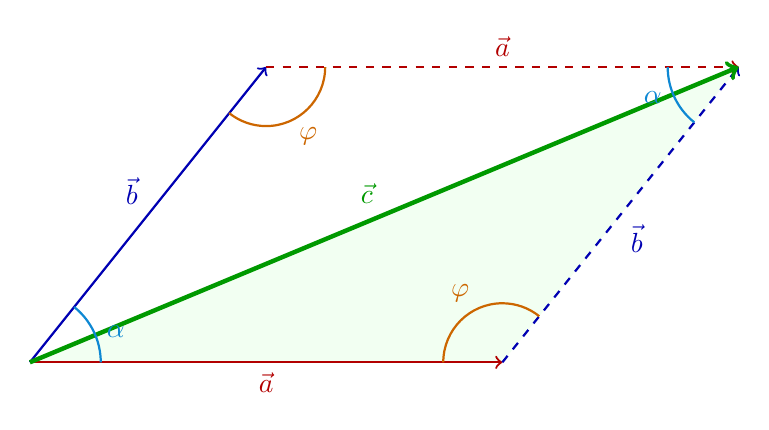
\begin{tikzpicture}[scale=1.5]
                \coordinate (O) at (0,0);
                \coordinate (A) at (4,0);
                \coordinate (B) at (2,2.5);
                \coordinate (C) at (6,2.5); % Resultante
            
                % Driehoek accentueren
                \fill[green!5] (O) -- (A) -- (C) -- cycle;
            
                % Het parallellogram
                \draw[->, thick, red!70!black] (O) -- (A) node[midway, below] {$\vec{a}$};
                \draw[->, thick, blue!70!black] (O) -- (B) node[midway, above left] {$\vec{b}$};
                \draw[->, dashed, thick, blue!70!black] (A) -- (C) node[midway, below right] {$\vec{b}$};
                \draw[->, dashed, thick, red!70!black] (B) -- (C) node[midway, above] {$\vec{a}$};
            
                % Resultante
                \draw[->, ultra thick, green!60!black] (O) -- (C) node[midway, above left] {$\vec{c}$};
            
                % Hoeken alpha (blauw)
                \draw[thick, cyan!70!blue] (0.6,0) arc (0:51.3:0.6) node[midway, right=1pt] {$\alpha$};
                \draw[thick, cyan!70!blue] (5.4,2.5) arc (180:231.3:0.6) node[midway, left=1pt] {$\alpha$};
            
                % Hoeken phi (oranje)
                \draw[thick, orange!80!black] (3.5,0) arc (180:51.3:0.5) node[midway, above left=-1pt] {$\varphi$};
                \draw[thick, orange!80!black] (2.5,2.5) arc (0:-128.7:0.5) node[midway, below right=-1pt] {$\varphi$};
            \end{tikzpicture}
            \captionof{figure}{De som van de hoeken in een parallellogram is $360^\circ$. Hierdoor zijn de vectorhoek $\alpha$ en de inwendige driehoekshoek $\varphi$ supplementair.}
            \label{fig:parallellogram_hoeken}
        \end{center}
        %---------------------------
    \end{hint}

\end{remark}

\begin{example}[title={Voorbeelden van vectoroptellingen}]\nl
    \textbf{Geval 1: Vectoren met dezelfde zin} \\
    Als $\|\vec{a}\| = 3\text{ N}$ en $\|\vec{b}\| = 5\text{ N}$, en ze wijzen in dezelfde richting, dan is $\| \vec{c} \| = \|\vec{a}\| + \|\vec{b}\| = 8\text{ N}$.
    
    \begin{center}
        \captionsetup{width=0.85\textwidth}
        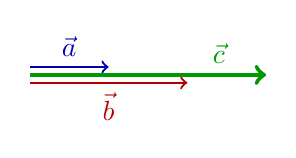
\begin{tikzpicture}[scale=1]
            \draw[->, thick, blue!70!black] (0,0.1) -- (1,0.1) node[midway, above]{$\vec{a}$};
            \draw[->, thick, red!70!black] (0,-0.1) -- (2,-0.1) node[midway, below]{$\vec{b}$};
            \draw[->, ultra thick, green!60!black] (0,0) -- (3,0) node[pos=0.8, above]{$\vec{c}$};
        \end{tikzpicture}
        \captionof{figure}{Vectoren met dezelfde zin.}
    \end{center}

    \textbf{Geval 2: Vectoren met tegengestelde zin} \\
    Als $\|\vec{a}\| = 3\text{ N}$ en $\|\vec{b}\| = 5\text{ N}$, maar ze wijzen in een tegengestelde zin, dan is $\| \vec{c} \| = | \|\vec{a}\| - \|\vec{b}\| | = 2\text{ N}$.
    
    \begin{center}
        \captionsetup{width=0.85\textwidth}
        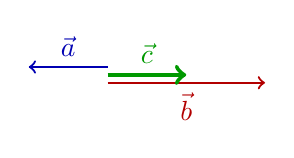
\begin{tikzpicture}[scale=1]
            \draw[->, thick, blue!70!black] (0,0.1) -- (-1,0.1) node[midway, above]{$\vec{a}$};
            \draw[->, thick, red!70!black] (0,-0.1) -- (2,-0.1) node[midway, below]{$\vec{b}$};
            \draw[->, ultra thick, green!60!black] (0,0) -- (1,0) node[midway, above]{$\vec{c}$};
        \end{tikzpicture}
        \captionof{figure}{Vectoren met tegengestelde zin.}
    \end{center}

    \textbf{Geval 3: Algemeen geval (Cosinusregel)} \\
    Als $\|\vec{a}\| = 3\text{ N}$, $\|\vec{b}\| = 5\text{ N}$ en de hoek ertussen $\alpha = 50^\circ$, bereken je de resultante via:
    \[ \|\vec{c}\| = \sqrt{3^2 + 5^2 + 2 \cdot 3 \cdot 5 \cdot \cos(50^\circ)} \approx 7,3\text{ N} \]

    De \textbf{richting van de resultante} (de hoek $\gamma$ met vector $\vec{b}$) kan bepaald worden met de sinusregel: 
    \[ \frac{\sin(\gamma)}{\|\vec{a}\|} = \frac{\sin(180^\circ-\alpha)}{\|\vec{c}\|} \quad \Longrightarrow \quad \sin(\gamma) = \frac{\|\vec{a}\|\sin(\alpha)}{\|\vec{c}\|} \]
    \[ \gamma = \arcsin\left(\frac{3 \cdot \sin(50^\circ)}{7,3}\right) \approx 18^\circ \]
\end{example}

\begin{remark}
    De optelling van vectoren is \textit{associatief}, d.w.z. dat $(\vec{a} + \vec{b}) + \vec{c} = \vec{a} + (\vec{b} + \vec{c})$. Indien er dus meer dan twee vectoren worden samengesteld, tel je er eerst twee op, en dat resultaat tel je op bij de volgende, enzovoort.
\end{remark}

\end{document}